\documentclass[shownotes,12pt, aspectratio=169]{beamer}
\usepackage{pgfpages}
% These slides also contain speaker notes. You can print just the slides,
% just the notes, or both, depending on the setting below. Comment out the want
% you want.
\setbeameroption{hide notes} % Only slide
%\setbeameroption{show only notes} % Only notes
%\setbeameroption{show notes on second screen=right} % Both
\usepackage[normalem]{ulem}
\usepackage{better-beamer}
\usepackage[OT1]{fontenc}
\renewcommand*\familydefault{\ttdefault}
\usepackage{array}
\usepackage{listings}
\usepackage{tikz}
\usepackage{verbatim}
\setbeamertemplate{note page}{\pagecolor{yellow!5}\insertnote}
\usetikzlibrary{positioning}
\usetikzlibrary{decorations.pathmorphing}
\usetikzlibrary{calc}
\usetikzlibrary{arrows}
\usetikzlibrary{decorations.markings}
\usetikzlibrary{shapes.misc}
\usetikzlibrary{matrix,shapes,arrows,fit,tikzmark}
\usepackage{amsmath}
\usepackage{mathpazo}
\usepackage{hyperref}
\usepackage{lipsum}
\usepackage{multimedia}
\usepackage{graphicx}
\usepackage{multirow}
\usepackage{graphicx}
\usepackage{dcolumn}
\usepackage{bbm}
\newcolumntype{d}[0]{D{.}{.}{5}}

\usepackage{changepage}
\usepackage{appendixnumberbeamer}
\newcommand{\beginbackup}{
   \newcounter{framenumbervorappendix}
   \setcounter{framenumbervorappendix}{\value{framenumber}}
   \setbeamertemplate{footline}
   {
     \leavevmode%
     \hline
     box{%
       \begin{beamercolorbox}[wd=\paperwidth,ht=2.25ex,dp=1ex,right]{footlinecolor}%
%         \insertframenumber  \hspace*{2ex}
       \end{beamercolorbox}}%
     \vskip0pt%
   }
 }
\newcommand{\backupend}{
   \addtocounter{framenumbervorappendix}{-\value{framenumber}}
   \addtocounter{framenumber}{\value{framenumbervorappendix}}
}
\usepackage{graphicx}
\usepackage[space]{grffile}
\usepackage{booktabs}

\title[]{\textcolor{blue}{Basic Data Vizualization}}
\author{Joshua F. Allen}
\date{\today}
% These are my colors -- there are many like them, but these ones are mine.
\definecolor{blue}{RGB}{50,87,86}
\definecolor{red}{RGB}{213,94,0}
\definecolor{yellow}{RGB}{240,228,66}
\definecolor{green}{RGB}{0,158,115}

\hypersetup{
  colorlinks=false,
  linkbordercolor = {white},
  linkcolor = {blue}
}


%% I use a beige off white for my background
\definecolor{MyBackground}{RGB}{255,253,218}

%% Uncomment this if you want to change the background color to something else
%\setbeamercolor{background canvas}{bg=MyBackground}

%% Change the bg color to adjust your transition slide background color!
\newenvironment{transitionframe}{
  \setbeamercolor{background canvas}{bg=yellow}
  \begin{frame}}{
    \end{frame}}

\setbeamercolor{frametitle}{fg=blue}
\setbeamercolor{title}{fg=black}
\setbeamertemplate{footline}[frame number]
\setbeamertemplate{navigation symbols}{}
\setbeamertemplate{itemize items}{-}
\setbeamercolor{itemize item}{fg=blue}
\setbeamercolor{itemize subitem}{fg=blue}
\setbeamercolor{enumerate item}{fg=blue}
\setbeamercolor{enumerate subitem}{fg=blue}
\setbeamercolor{button}{bg=MyBackground,fg=blue,}



% If you like road maps, rather than having clutter at the top, have a roadmap show up at the end of each section
% (and after your introduction)
% Uncomment this is if you want the roadmap!
% \AtBeginSection[]
% {
%    \begin{frame}
%        \frametitle{Roadmap of Talk}
%        \tableofcontents[currentsection]
%    \end{frame}
% }
\setbeamercolor{section in toc}{fg=blue}
\setbeamercolor{subsection in toc}{fg=red}
\setbeamersize{text margin left=1em,text margin right=1em}

\newenvironment{wideitemize}{\itemize\addtolength{\itemsep}{10pt}}{\enditemize}

\usepackage{environ}
\NewEnviron{videoframe}[1]{
  \begin{frame}
    \vspace{-8pt}
    \begin{columns}[onlytextwidth, T] % align columns
      \begin{column}{.58\textwidth}
        \begin{minipage}[t][\textheight][t]
          {\dimexpr\textwidth}
          \vspace{8pt}
          \hspace{4pt} {\Large \sc \textcolor{blue}{#1}}
          \vspace{8pt}

          \BODY
        \end{minipage}
      \end{column}%
      \hfill%
      \begin{column}{.42\textwidth}
        \colorbox{green!20}{\begin{minipage}[t][1.2\textheight][t]
            {\dimexpr\textwidth}
            Face goes here
          \end{minipage}}
      \end{column}%
    \end{columns}
  \end{frame}
}
\begin{document}

\tikzset{
        every picture/.style={remember picture,baseline},
        every node/.style={anchor=base,align=center,outer sep=1.5pt},
        every path/.style={thick},
        }
\newcommand\marktopleft[1]{%
    \tikz[overlay,remember picture]
        \node (marker-#1-a) at (-.3em,.3em) {};%
}
\newcommand\markbottomright[2]{%
    \tikz[overlay,remember picture]
        \node (marker-#1-b) at (0em,0em) {};%
}
\tikzstyle{every picture}+=[remember picture]
\tikzstyle{mybox} =[draw=black, very thick, rectangle, inner sep=10pt, inner ysep=20pt]
\tikzstyle{fancytitle} =[draw=black,fill=red, text=white]
%%%% END TIKZ STUFF


% Title Slide
\begin{frame}

\maketitle

\end{frame}
%--- Next Frame ---%

\section{Data Vizualization a Crash Course}
\begin{transitionframe}
  \begin{center}
    \Huge Why This is Important
  \end{center}
\end{transitionframe}

% ------------------------------------------
\begin{frame}[t]{Why Can't I Just use Summary Stats?}
  \begin{itemize}
    \item Measures of centeral tendency are vital for exploratory analysis
    \item They tell you a lot about your data
    \pause
    \item However, they can not reveal patterns
  \end{itemize}
\end{frame}
\note[itemize]{
\item Getting to know your data is super important because you need to know what you can do and what you need to do.
\item You get a base understaning of it through summary statistics

}
%--- Next Frame ---%
\begin{frame}[t]{Going Beyond Summary stats}
  \begin{center}
  \resizebox{0.58\linewidth}{!}{
   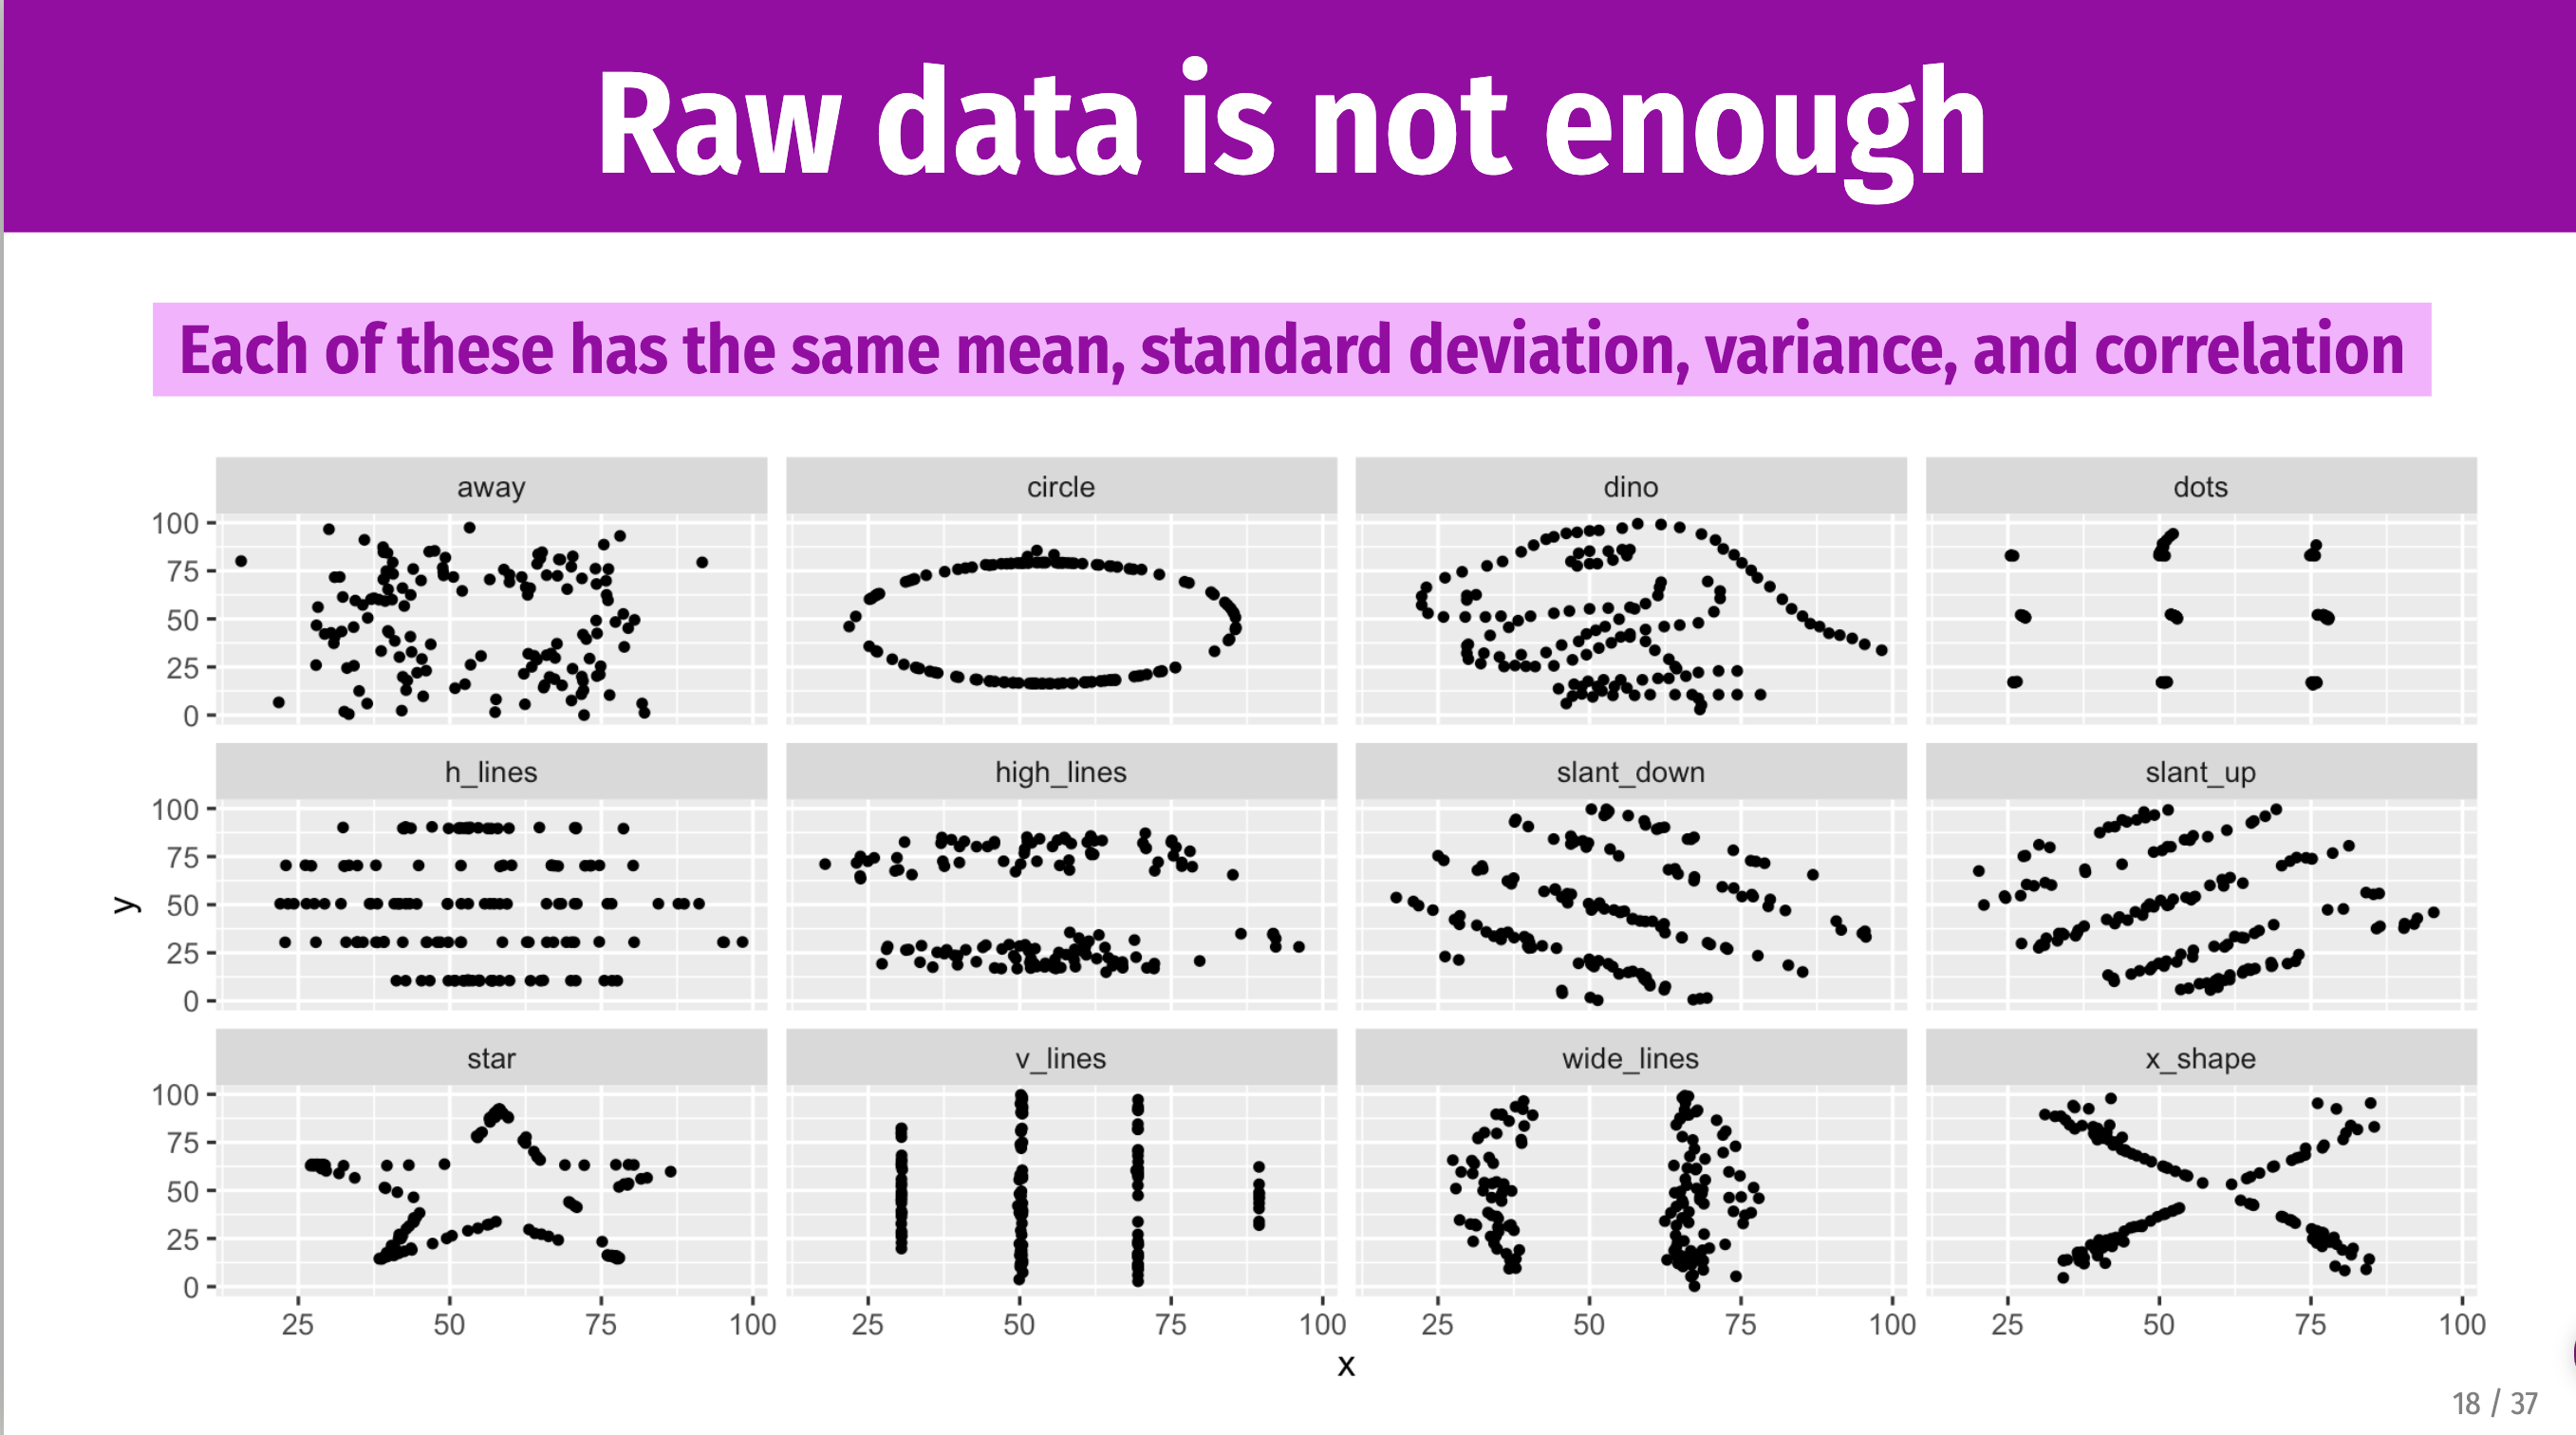
\includegraphics{andrew-slide.png}
 }
\end{center}
\end{frame}
\note[itemize]{
\item this is a play on what is known as Anscombe's quartet.
\item each of these graphs have the sameish summary stats with slight differenences on the very tails.
\item if you just use summary stats you aren't seeing the patterns in your data. We as humans are good at picking out patterns. Most of us are really bad at looking at a spreadsheet and figuring out patterns in it.
}

\transreplace
\begin{frame}[t]{Going Beyond Summary stats}
  \begin{center}
  \resizebox{0.5\linewidth}{!}{
   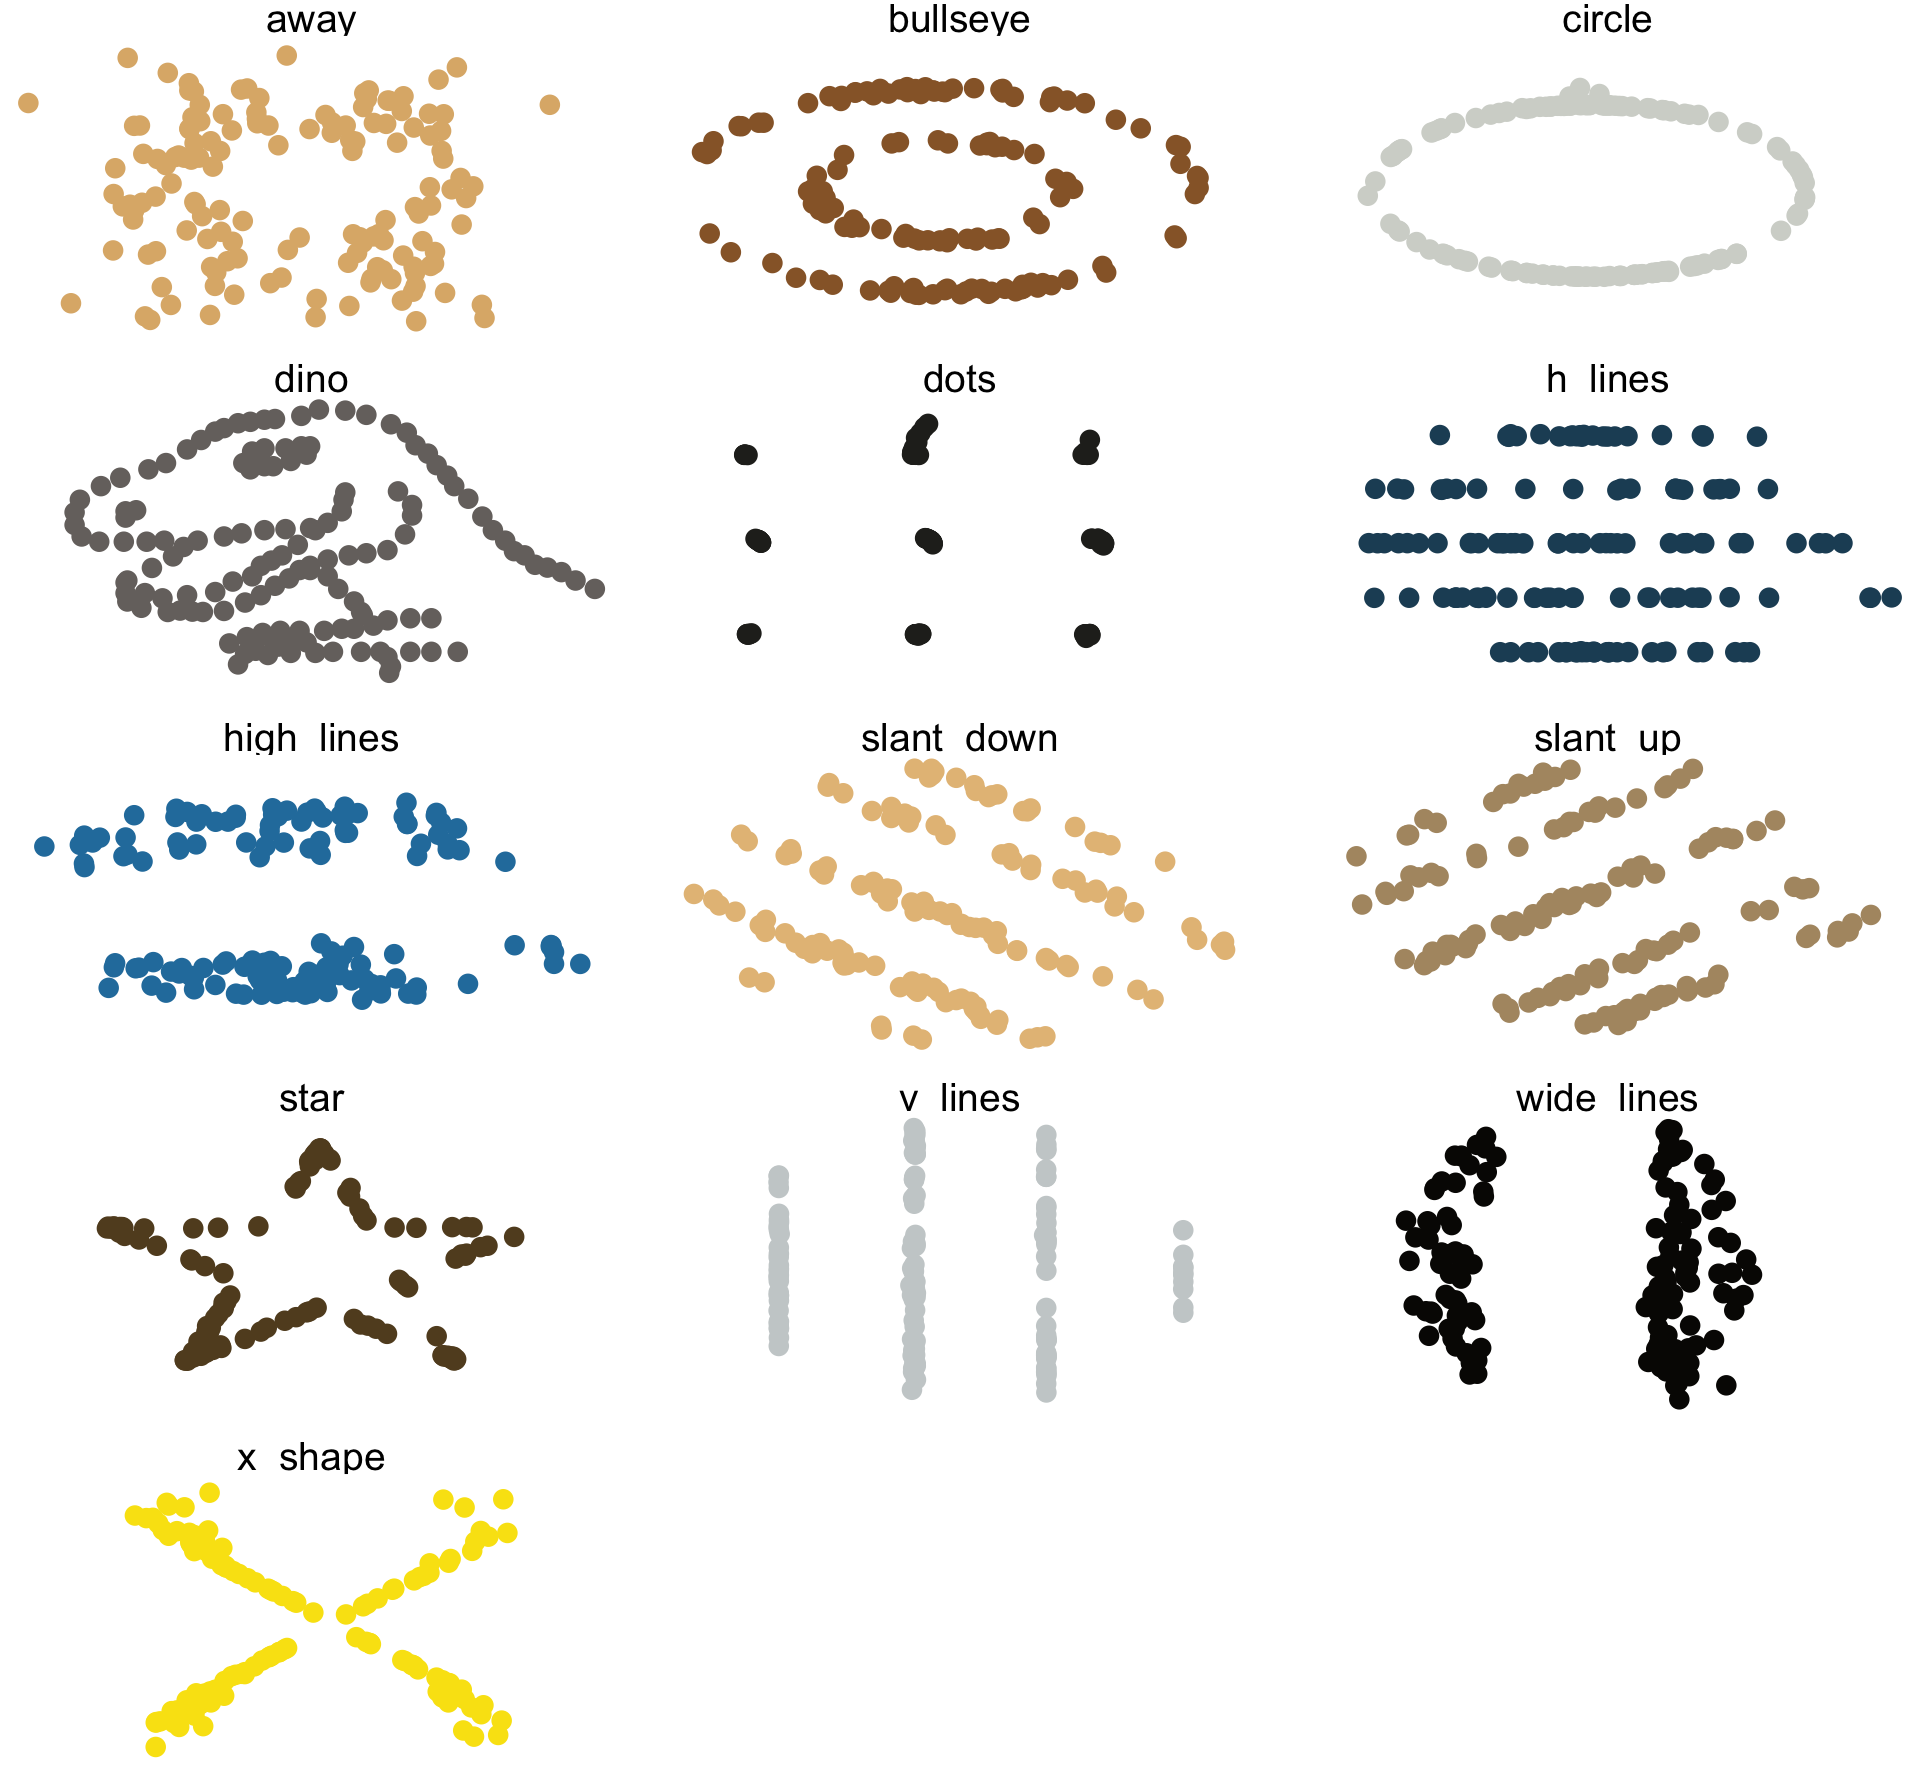
\includegraphics{dinoplot.png}
 }
\end{center}
\end{frame}


\begin{frame}[t]{What Makes a Good Vizualization?}
  \begin{itemize}
    \item People have lots of opinions
    \item Books are dedicated to this
    \item This is a legit topic scholars debate
  \end{itemize}
\end{frame}
%--- Next Frame ---%
 \note[itemize]{
 \item I am doing a surface level coverage of a huge debate
 \item I often joke that data viz is art for people wih no artistic talent.
 \item It is a skill that will make you stand out at the work place
 }

\begin{frame}[t]{The Basics}
  \begin{itemize}
    \item Faithful representation of the data
    \item Good Aesthics
    \item No perceptual issues
    \item Insightful
  \end{itemize}
\end{frame}
\note[itemize]{
\item The most important part of sort of "rule" for dataviz is that you are honest.
\item  the data are accurate as it can be, you are not letting the data tell you things. Data will lie to you if you don't choose the right measures. One example of this was a sort of an alarmist story a few years ago that
\item Perceptual issues contains a lot. This can include issue related to colorblindness, low vision. Others are as minor as whether you have the right aspect ratio.
\item I usually think of insightful as having two aspects to it. Bang for your buck and whether the audience gets something out of it they otherwise wouldn't. Essentially just the dinograph example.

}




\begin{frame}[t]{Bad Data Vizualization}
  \begin{center}
  \resizebox{0.5\linewidth}{!}{
   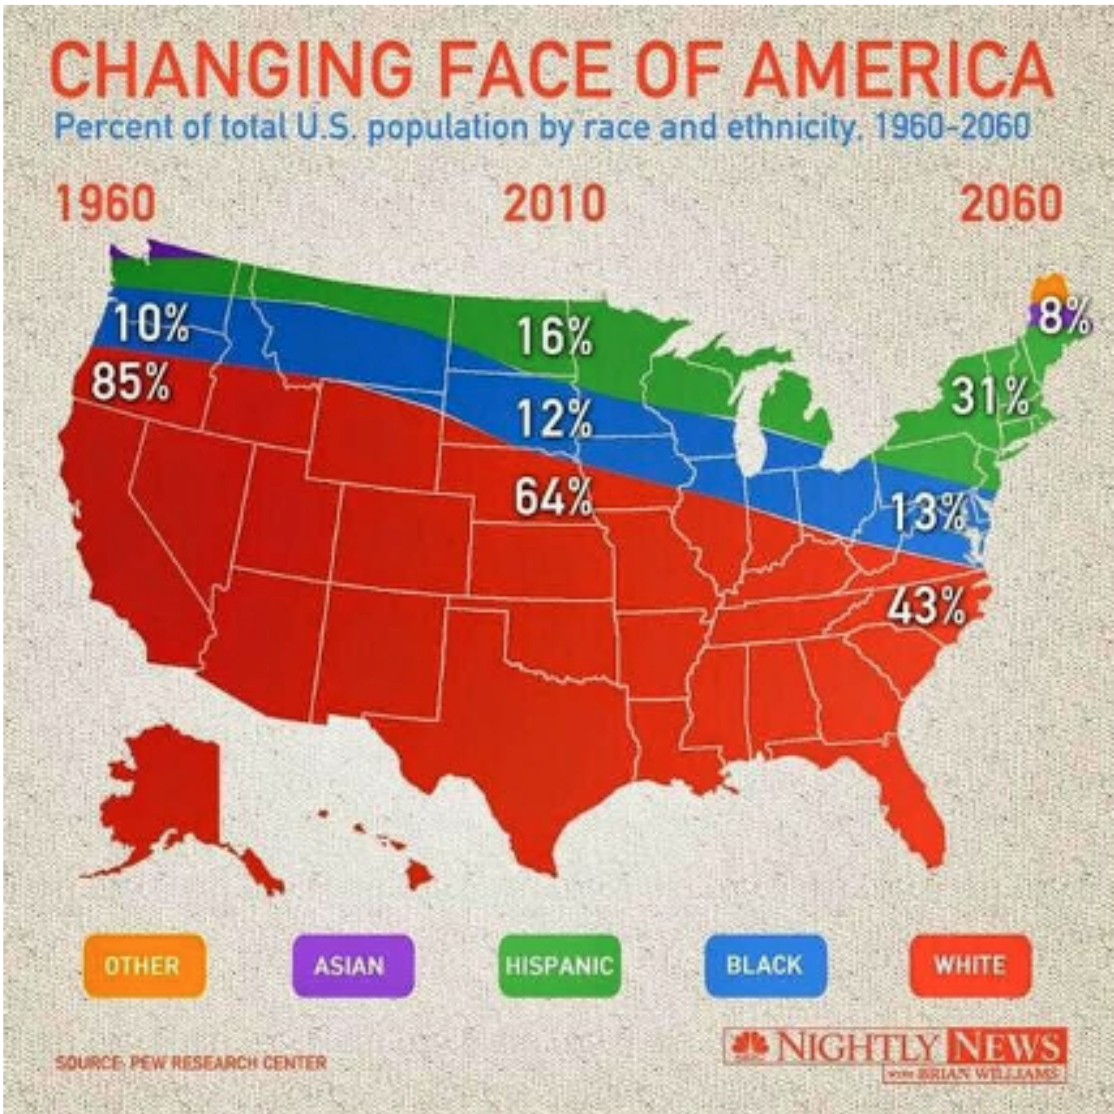
\includegraphics{bad.png}
 }
\end{center}
\end{frame}

\note[itemize]{
\item The contrast is .
\item that is the only thing that is going for it.
\item the graph implies that it represents spacial variation which is not true
\item we can not understand what is going on in the corners.
\item there are better ways to do this.
}

\begin{frame}[t]{Minard's Map}
  \begin{center}
  \resizebox{0.9\linewidth}{!}{
   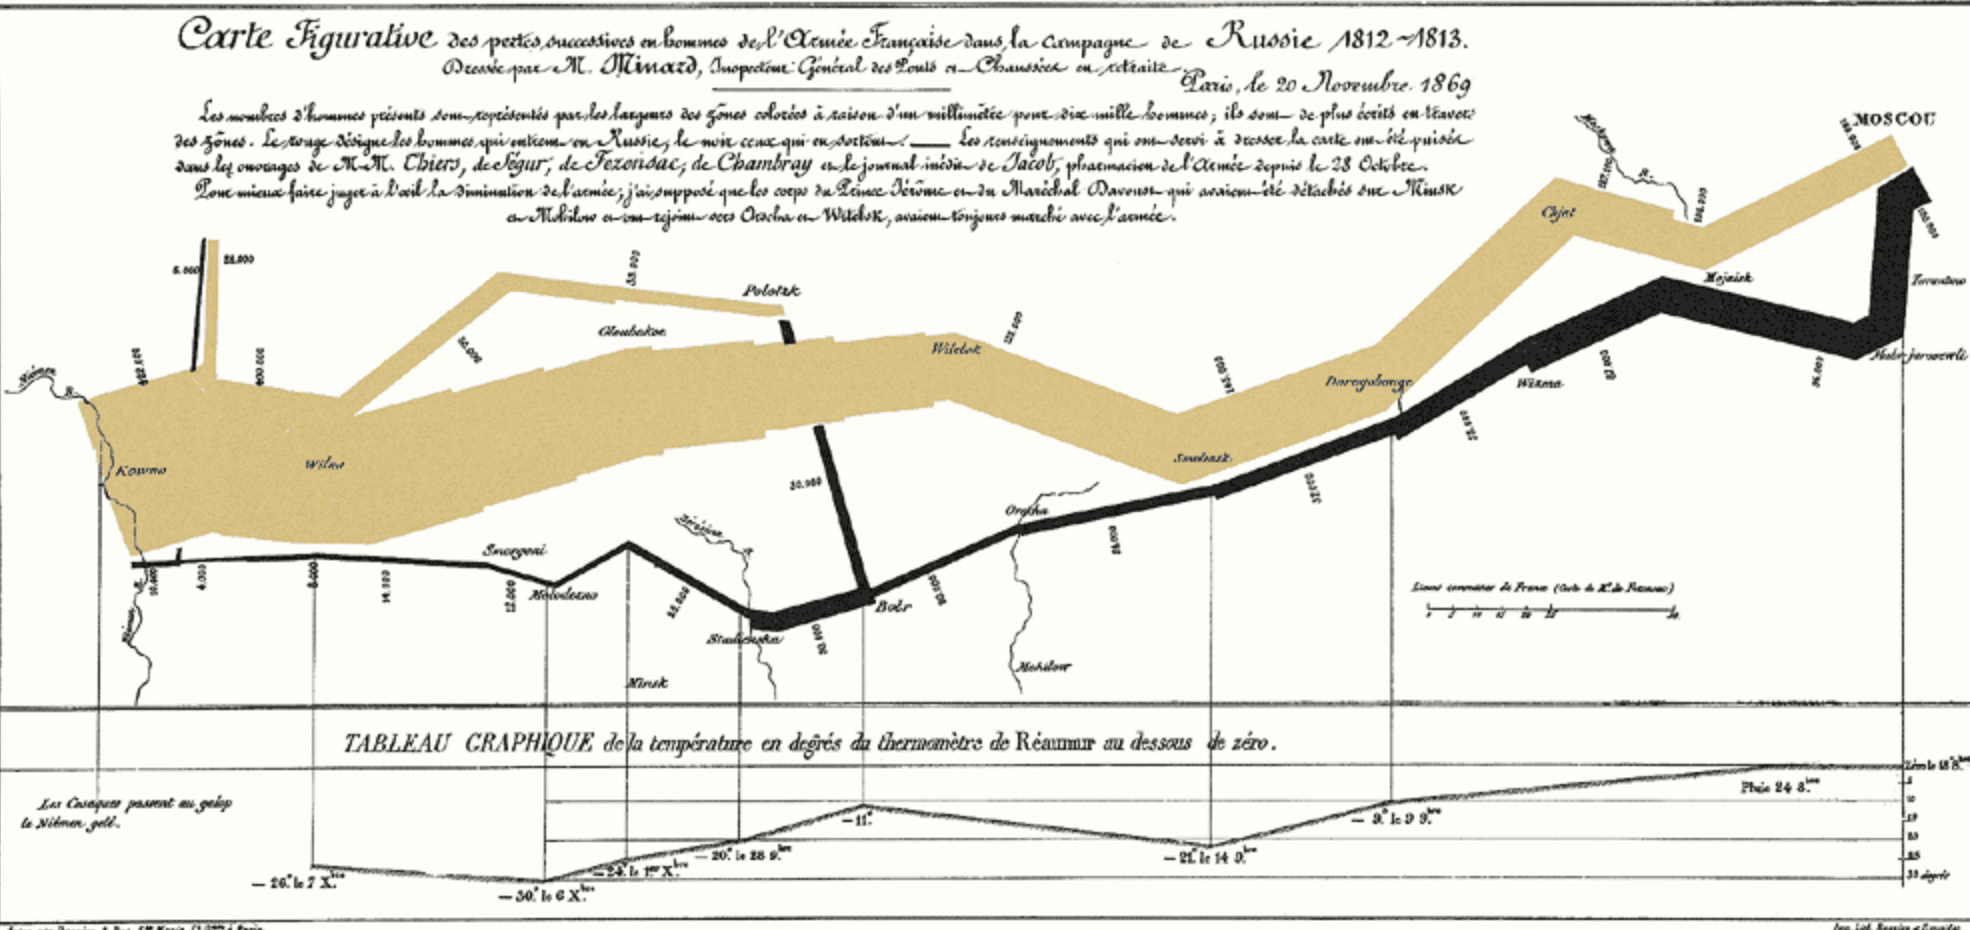
\includegraphics{minard.png}
 }
\end{center}
\end{frame}
\note[itemize]{
\item
\item Minard visualized Napolean's March to Russia and back from Russia and is often held up as the best data vizualization by the father of modern data viz Edward Tufte
\item Lets walk through it.
\item the brown line is the march to Russia and the Black line represents the . In both black and the brown bars the width represents the number of troops 1mm for every 10,000 troops.
\item There are also little tick marks indicating the number of troops.
\item You also have a sort of exact route demarked by major cities.
\item At the bottom you have how cold it is when winter hits.
\item The author also acknowledges some its inacurricies in the notes.
}
%--- Next Frame ---%
\section{Coding}
\begin{transitionframe}
  \begin{center}
\Huge Coding
\end{center}
\end{transitionframe}

\begin{frame}[t]{Should I Learn to Code?}
\begin{itemize}
  \item STATA, SAS, Excel, and SPSS have dropdown menus
  \pause
  \item You can get away with never learning the basics
  \pause
  \item It's really easy to do it that way..Kind of
\end{itemize}
\end{frame}
\note[itemize]{
\item Widely used tools like SAS, excel and SPSS give you the option to point and click your way to glory. There is nothing inherently wrong with this.
\item Thats how I started and would end up just copying the code into my do file.
\item It is super easy however it can come at some costs.
}
%--- Next Frame ---%
\begin{frame}[t]{Coding Continued}
\begin{columns}
\begin{column}[T]{0.5\textwidth}
  \resizebox{0.7\linewidth}{!}{
        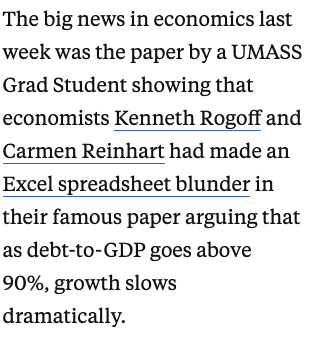
\includegraphics{excel.png}}
\end{column}
\hfill
\begin{column}[T]{0.5\textwidth}
  \begin{wideitemize}
     \item[-] It is \textcolor{red}{bad} practice to do stuff in the console or by drop downs
     \item[-] It leads to mistakes
     \item[-] And you won't ever really remember how to do things
   \end{wideitemize}
\end{column}
\end{columns}

\end{frame}

\note[itemize]{

\item This is a fairly recent example of when things go wrong
\item two notable economists published a paper in a fairly influential journal
\item but their results were very wrong because amongst other things they were
dragging down to the bottom of their excel
\item ultimately it also will just take longer for you to do things to. It is a
slow process
}

%--- Next Frame ---%

\begin{frame}[fragile]{Try Recreating this Figure}
\begin{columns}
\begin{column}[T]{0.5\textwidth}
    \resizebox{\textwidth}{!}{%
    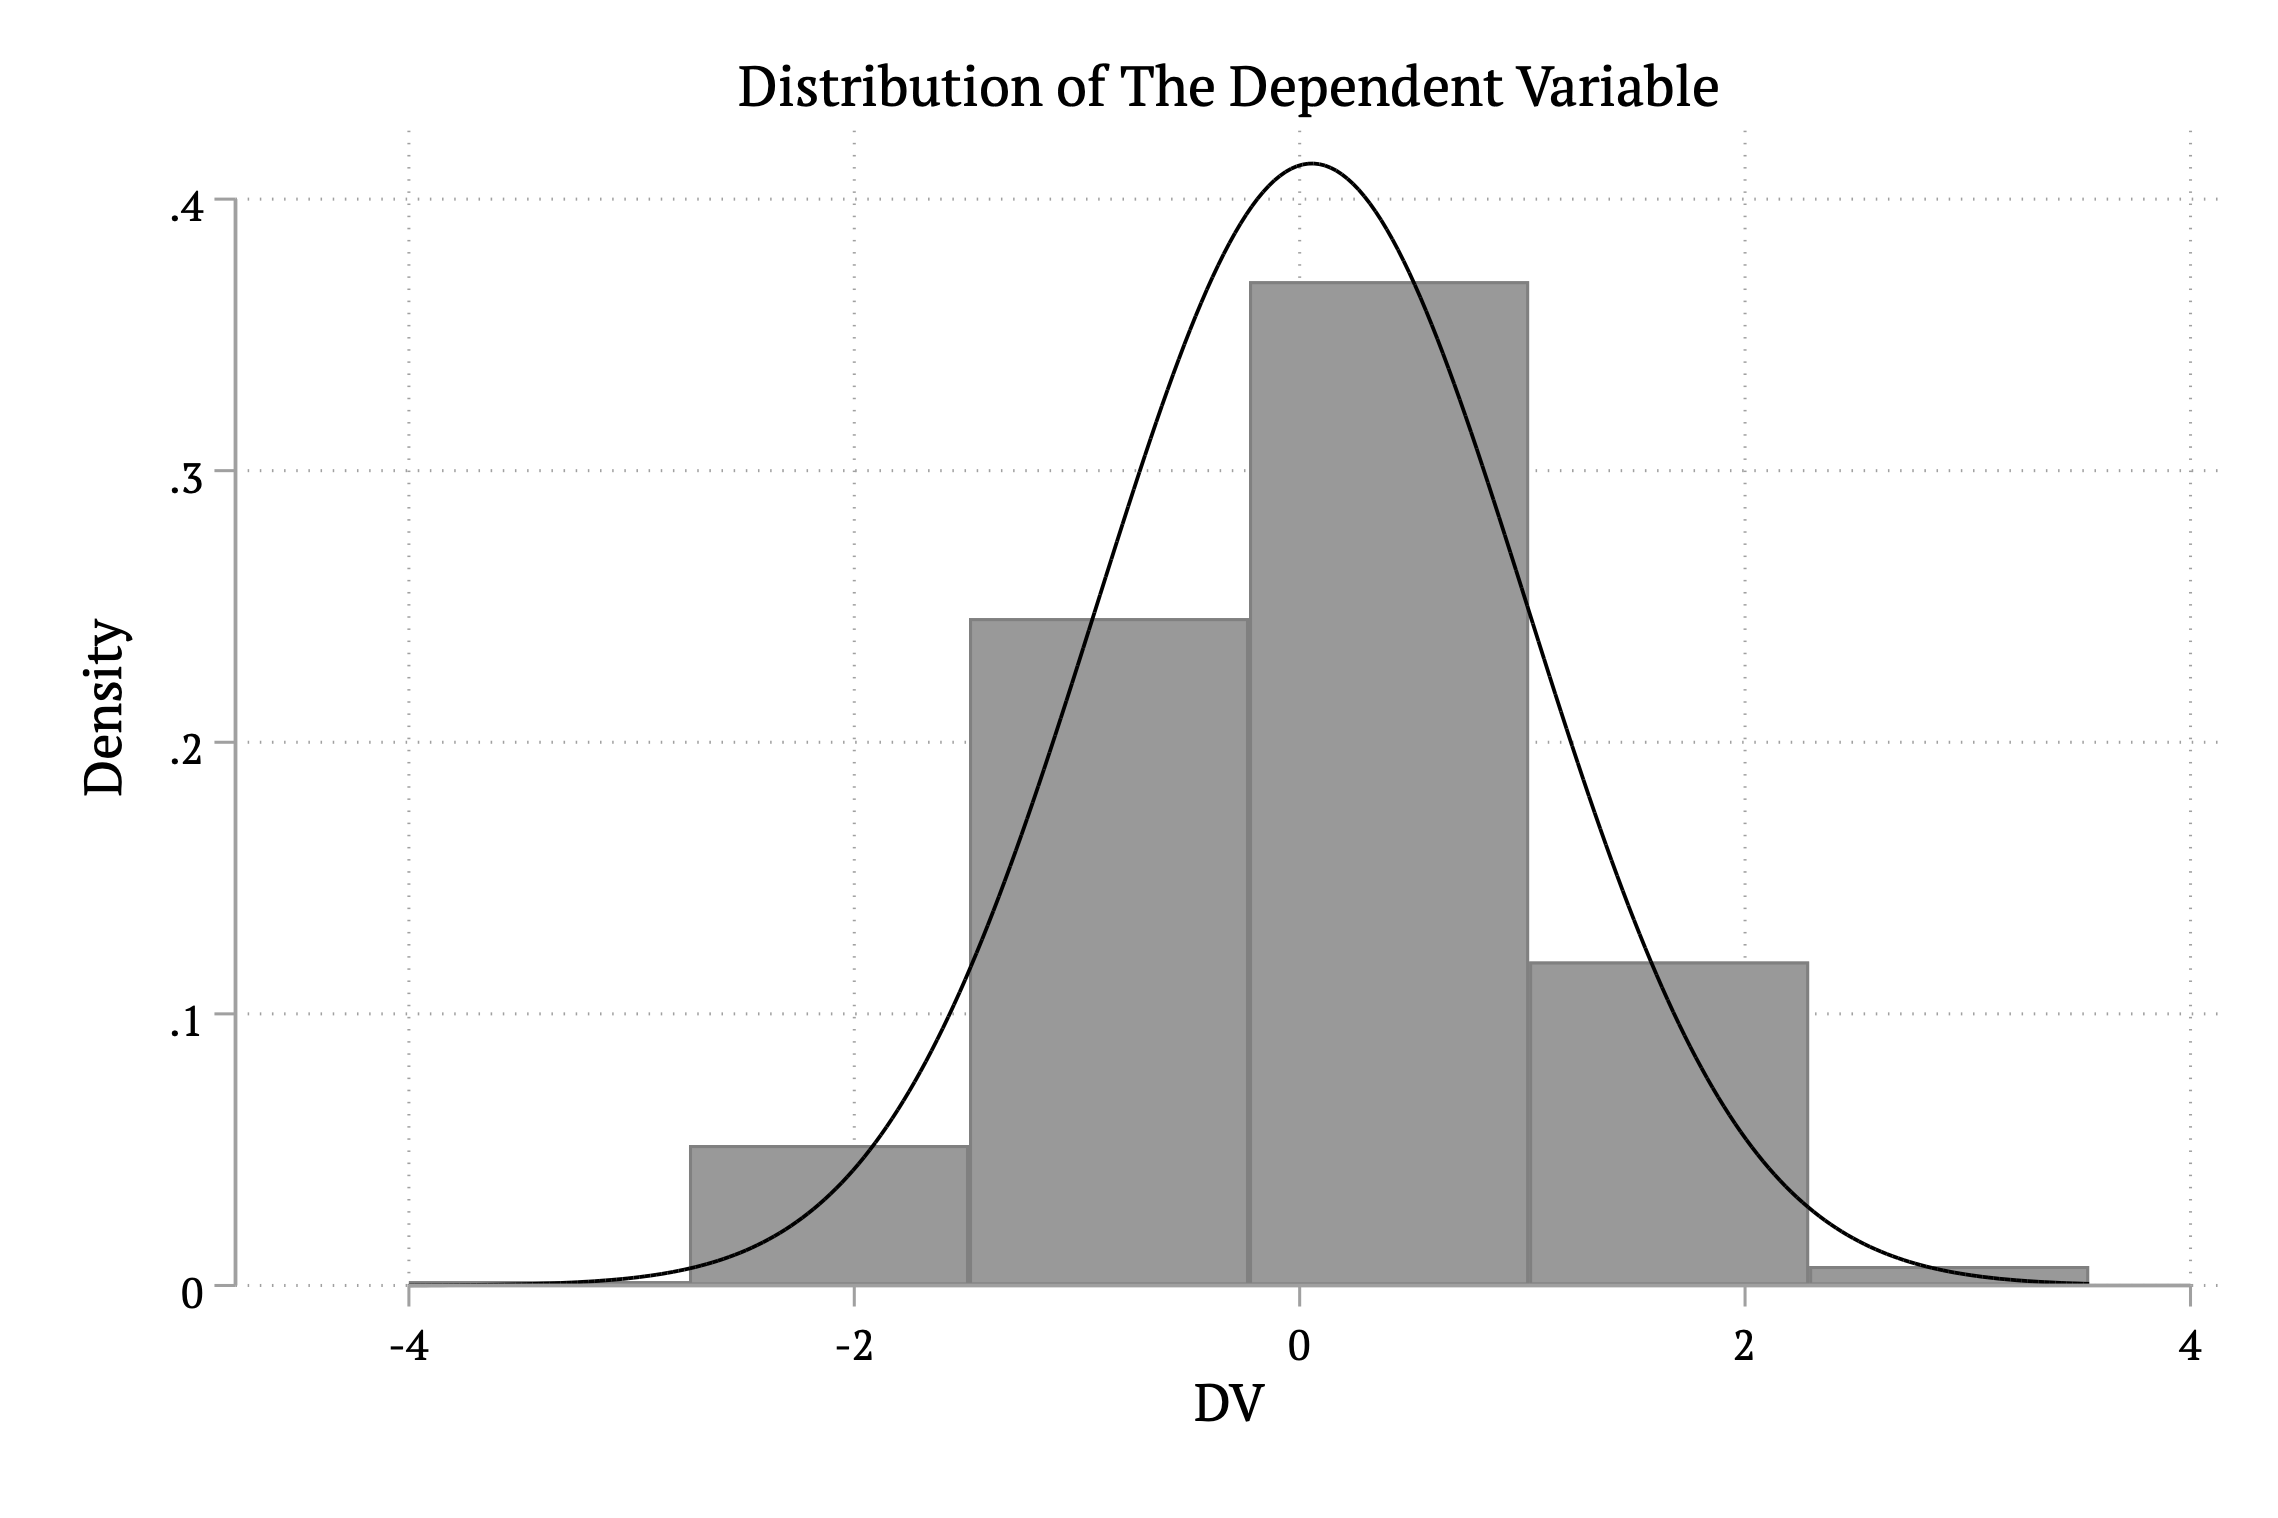
\includegraphics{hist.png}}
\end{column}
\hfill
\begin{column}{0.5\textwidth}
\begin{verbatim}

clear
*this will generate fake data
set seed 1994

set obs 1000

 g y = rnormal(0,1) /* mean = 0, sd = 1 */



\end{verbatim}
\end{column}
\end{columns}
\end{frame}
%--- Next Frame ---%
\begin{frame}[t]{How I created this figure}
\begin{columns}
\begin{column}[T]{0.5\textwidth}
    \resizebox{\textwidth}{!}{
    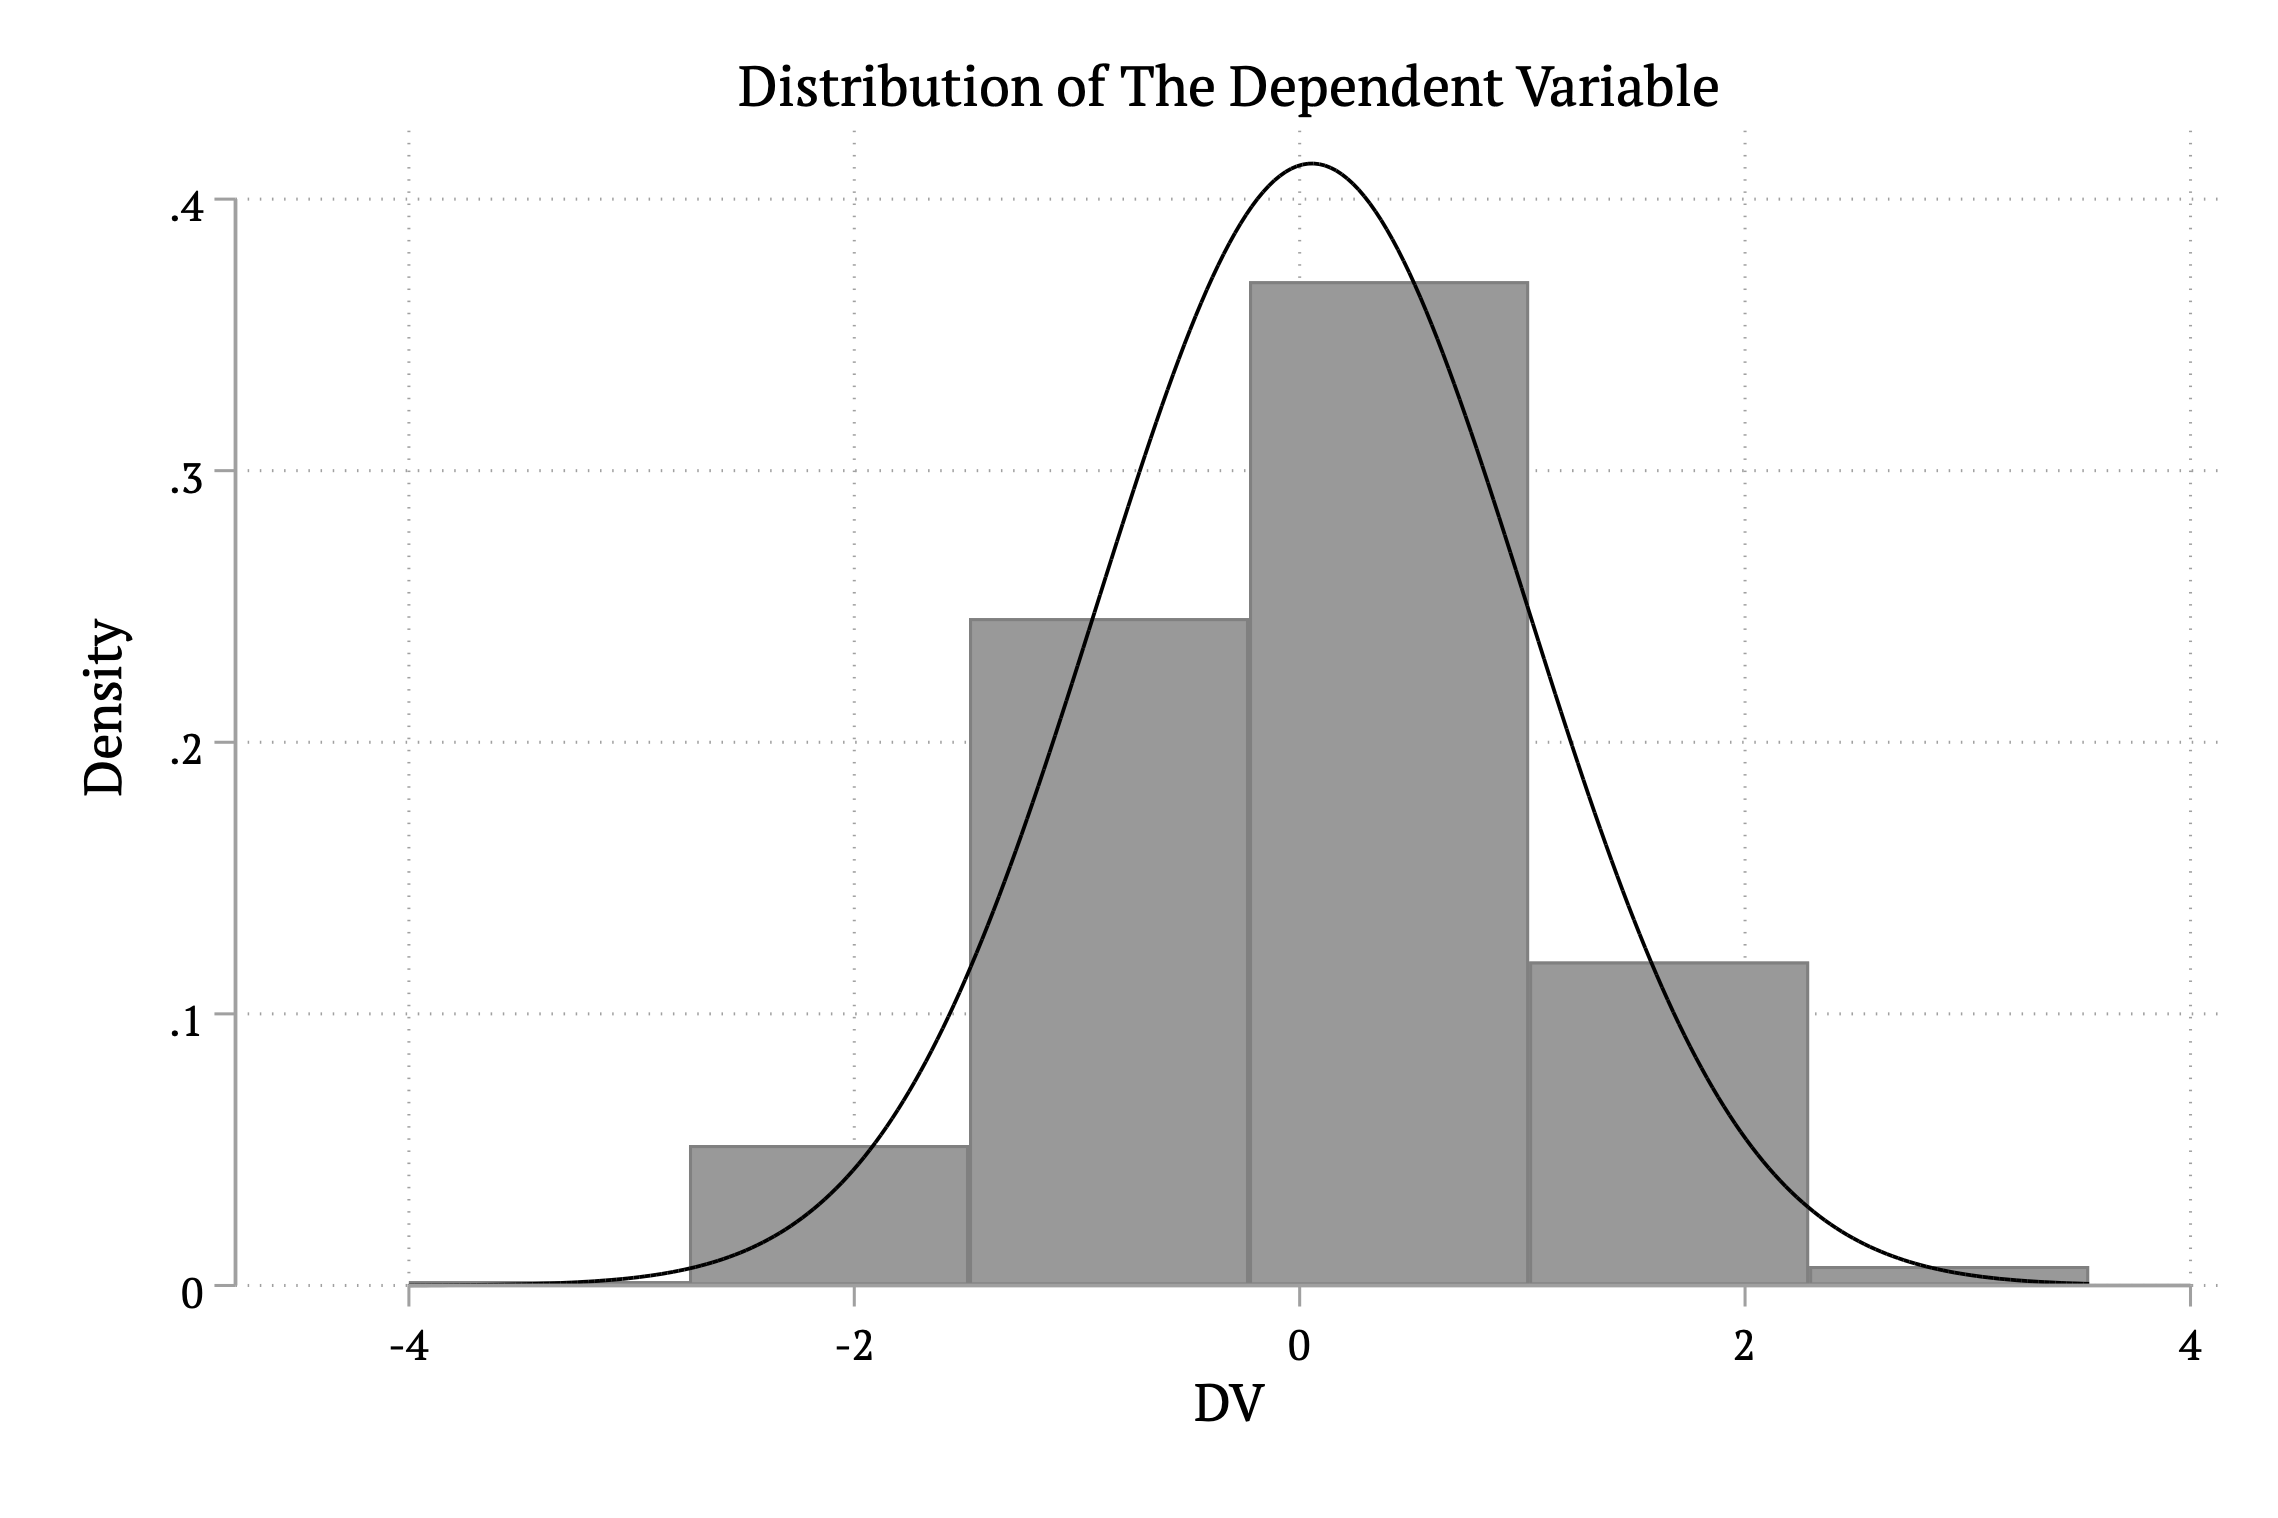
\includegraphics{hist.png}}
\end{column}
\hfill
\begin{column}{0.5\textwidth}
    \begin{verbatim}
      hist y, graphregion(color(white)) bin(6) bcolor(gs8 start(-4) normal ///
xtitle("DV") title("Distribution of The Dependent Variable") ///
normopts(lcolor(black))
    \end{verbatim}
\end{column}
\end{columns}
\end{frame}

\begin{frame}[t]{Learning To Code}
  \begin{wideitemize}
  \item It is hard and often frustrating at first.
  \pause
  \item You got this
  \item Understanding the fundamentals will let you do a lot of things.
  \end{wideitemize}
\end{frame}


\begin{frame}[t]{Resources}
\begin{columns}
\begin{column}[T]{0.5\textwidth}
  \resizebox{0.7\linewidth}{!}{
        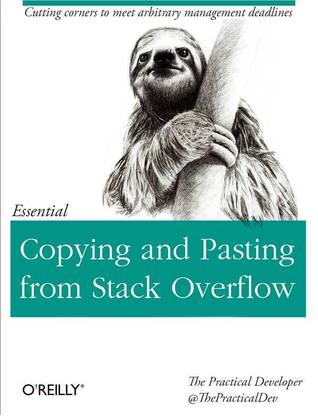
\includegraphics{stackoverflow.png}}
\end{column}
\hfill
\pause
\begin{column}[T]{0.5\textwidth}
  \resizebox{0.7\linewidth}{!}{
        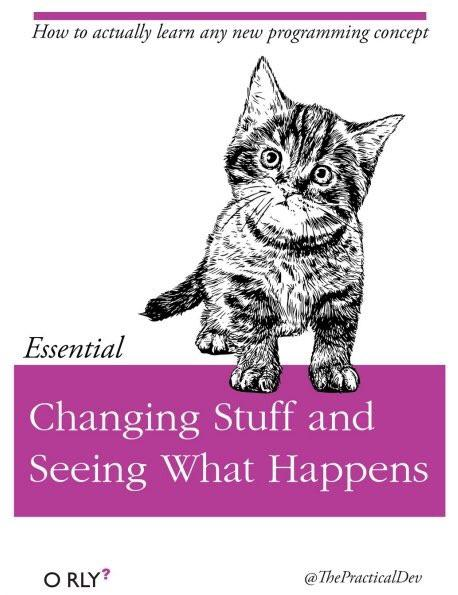
\includegraphics{stackoverflow2.png}}
\end{column}
\end{columns}
\end{frame}
\note[itemize]{
\item The internet is your friend.
\item For the most part when you are doing stuff in Stata and R that does not require you to build in additional security.
\item I learned by copy and pasting stuff then changing it and trying to figure out how I broke the code.
\item It is unreasonable to expect that you can memorize every command and to work through fixes yourself.
}


\section{Basics in Stata}

\begin{transitionframe}
  \begin{center}
\Huge Stata Basics
\end{center}
\end{transitionframe}


\begin{frame}[t]{Things to Keep in Mind When Making Graphs}
  \begin{itemize}
    \item Stata has notoriously ugly defaults
    \item Stata\textsuperscript{\tiny\textregistered} has lots of opinions about what you should not do
    \item All the graphing commands have similar syntax, but with slight tweaks
    \item These tweaks can cause you to get grumpy
    \pause
    \item Like really grumpy
  \end{itemize}
\end{frame}
%--- Next Frame ---%
\begin{frame}[t]{Basic Grammar}
\begin{columns}
\begin{column}[T]{.5\textwidth}
\begin{verbatim}

command varlist [if] [in], options

\end{verbatim}
\end{column}
\hfill
\begin{column}[T]{.5\textwidth}
\begin{itemize}
  \item "varlist" is a column in your dataset
  \item "if" is a set of conditional statements
  \item  "in" is usually a some rows in your dataset or used for weights
\end{itemize}
\end{column}
\end{columns}
\end{frame}

\section{Coding Time}


\begin{transitionframe}
  \begin{center}
\Huge Coding Time!
\end{center}
\end{transitionframe}

\begin{frame}[t]{Very Basics}
  \begin{itemize}
    \item The best practice is to have an \textbf{individual} folder for each project
    \item you should have Stata pointed at that folder
    \item this is done by cd "path/to/your/file" on Mac
  \end{itemize}
\end{frame}
%--- Next Frame ---%


\begin{frame}[t]{Default Stata Graph vs Highly Customized}
  \begin{columns}
  \begin{column}[T]{.5\textwidth}
    \begin{center}
  \resizebox{0.9\linewidth}{!}{%
  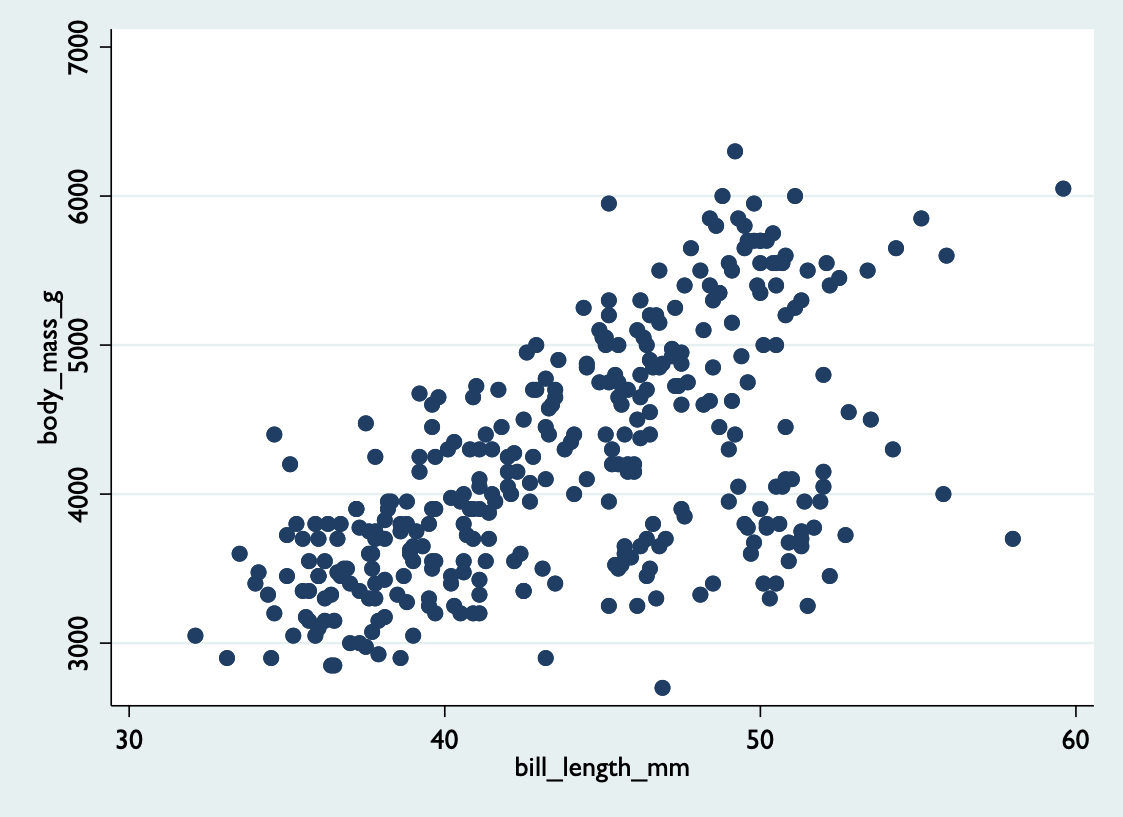
\includegraphics{penguin-basic.png}}
\end{center}
  \end{column}
\end{columns}
\end{frame}
  \transreplace
  \begin{frame}[t]{Default Stata Graph vs Highly Customized}
  \begin{columns}
  \begin{column}[T]{.5\textwidth}
    \begin{center}
    \resizebox{1.0\linewidth}{!}{%
    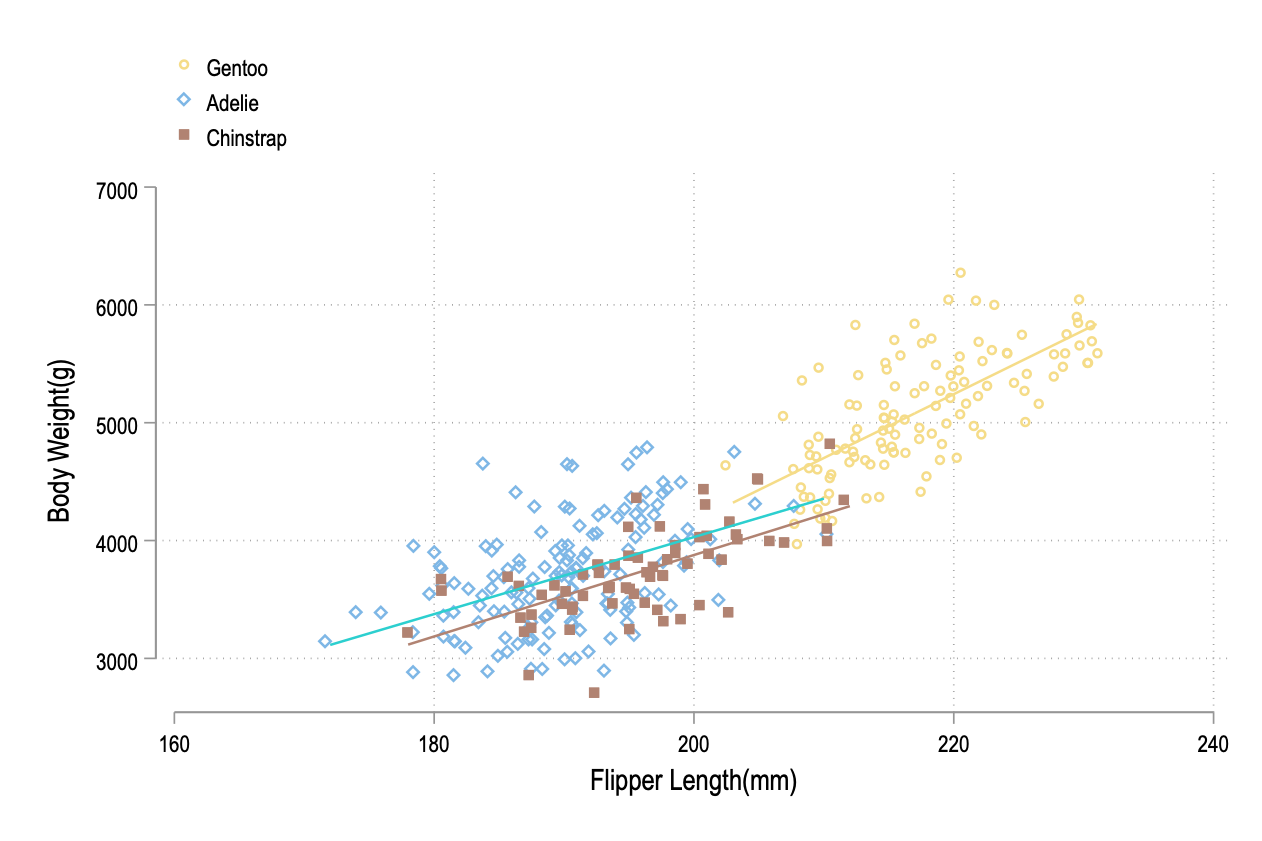
\includegraphics{penguins-manu-example.png}}
  \end{center}
  \end{column}
  \end{columns}

\end{frame}


%--- Next Frame ---%


%--- Next Frame ---%
%--- Next Frame ---%

\begin{frame}[t]{Why is it == and not =?}
  \begin{itemize}
    \item Stata uses what are called booleans
    \item "\&" is and
    \item "|" is or
    \item "!" is not.
    \item "==" is equal to
    \item "=" in most software languages is used for assignment
  \end{itemize}
\end{frame}



\begin{frame}[t]{Example of Assignment in Stata}
  \begin{columns}
  \begin{column}[T]{.5\textwidth}
  \begin{verbatim}

egen toy\_var = mean(other\_var)



  \end{verbatim}
  \end{column}
  \end{columns}

\end{frame}
%--- Next Frame ---%


\section{Appendix}
\begin{transitionframe}
  \begin{center}
\Huge Appendix
\end{center}
\end{transitionframe}

\begin{frame}[t]{Resources}
  \begin{itemize}
    \item \href{https://datavizm20.classes.andrewheiss.com/}{Open Source Course in R}
    \item \href{https://www.stata.com/bookstore/statacheatsheets.pdf}{Stata Cheat Sheet}
    \item \href{http://geocenter.github.io/StataTraining/}{Open Source Course for learning Stata}
  \end{itemize}
\end{frame}
%--- Next Frame ---%
\begin{frame}[t]{Manually Cleaning Up Stata Plots}
\begin{columns}
\begin{column}[T]{.5\textwidth}
  \begin{center}
\resizebox{0.8\linewidth}{!}{%
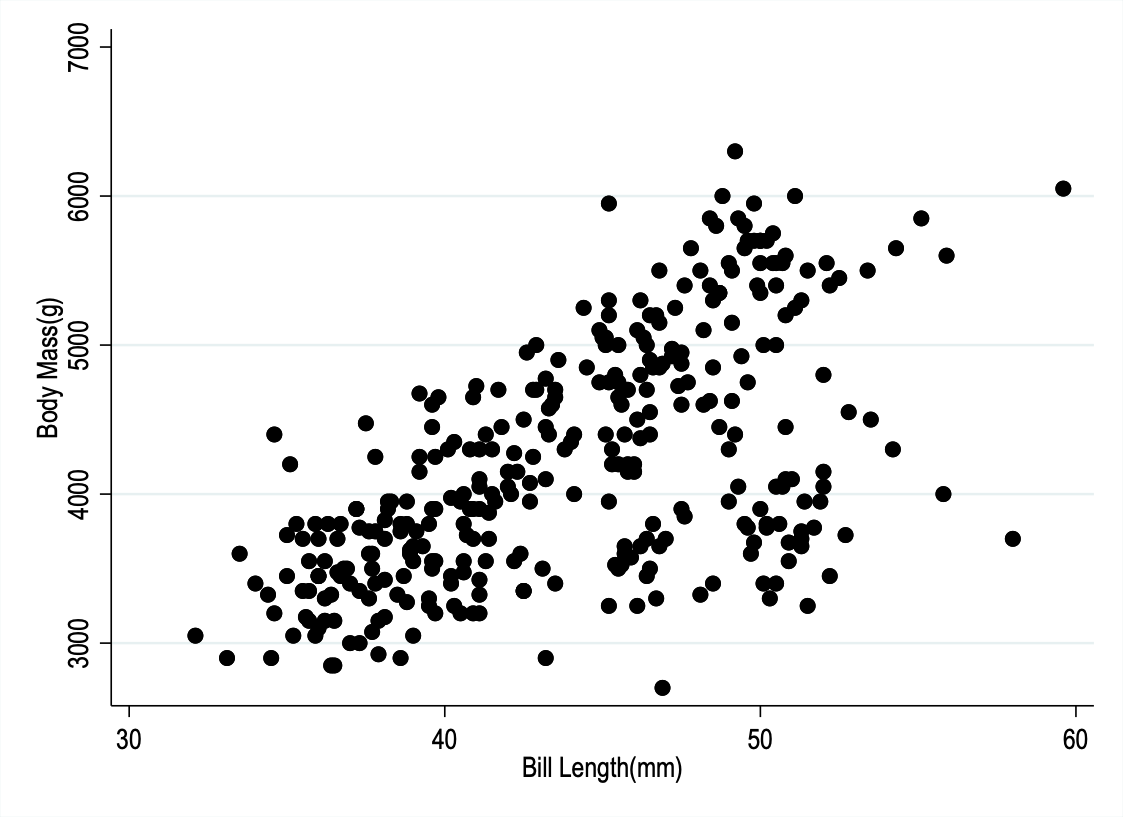
\includegraphics{penguin-basic-with-title.png}}
\end{center}
\end{column}
\hfill
\begin{column}[T]{.5\textwidth}
\begin{verbatim}

  tw scatter body\_mass\_g bill\_length\_mm, graphregion(color(white)) ///

   xtitle("Bill Length(mm)") ytitle("Body Mass(g)")  mcolor(black)
\end{verbatim}

\end{column}
\end{columns}

\end{frame}
%--- Next Frame ---%
\transreplace

\begin{frame}[t]{Notice How the Points Overlap?}
  \begin{columns}
  \begin{column}[T]{.5\textwidth}
    \begin{center}
  \resizebox{0.8\linewidth}{!}{%
  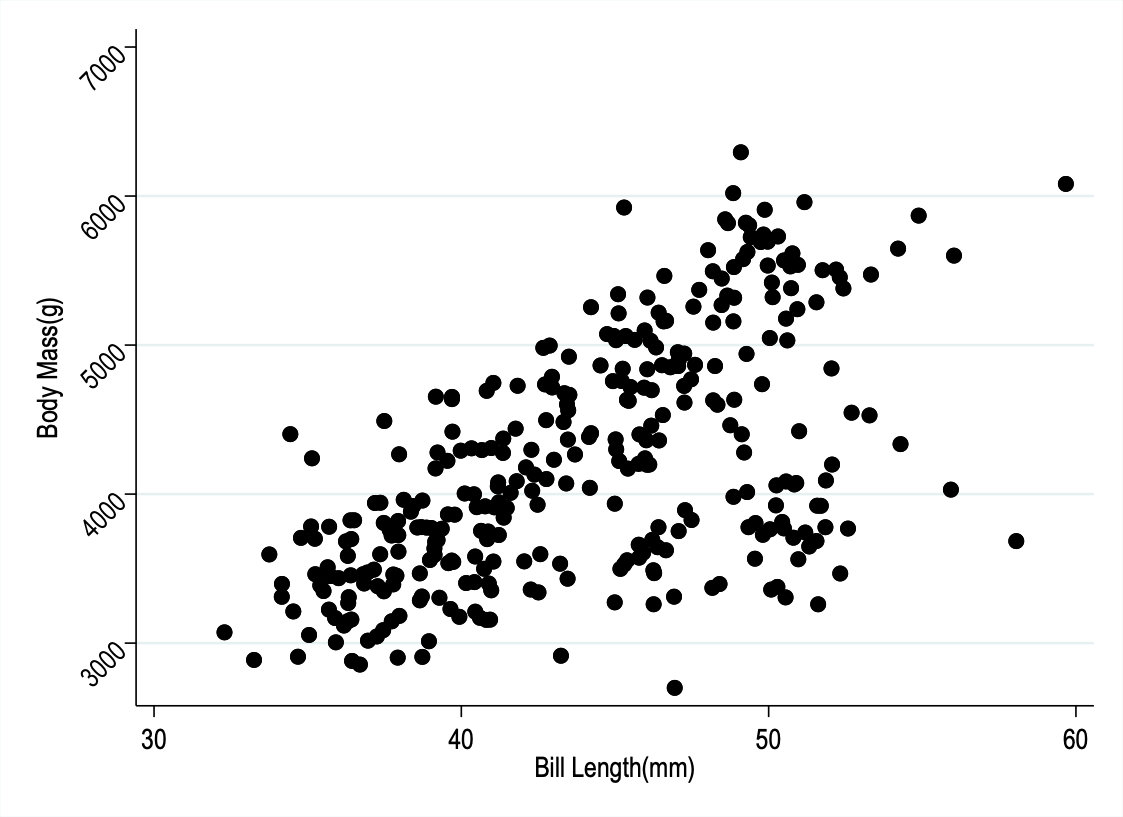
\includegraphics{scatter-penguins-jitter.png}}
  \end{center}
  \end{column}
  \hfill
  \begin{column}[T]{.5\textwidth}
  \begin{verbatim}

    tw scatter body\_mass\_g bill\_length\_mm, graphregion(color(white)) ///
    ylabel(,angle(45)) ///
     jitter(2) jitterseed(1994) xtitle("Bill Length(mm)") mclor(black)
  \end{verbatim}
  \end{column}
  \end{columns}
\end{frame}

\begin{frame}[t]{Conditional Statements}
  \begin{columns}
  \begin{column}[T]{.5\textwidth}
    \begin{center}
    \resizebox{0.8\linewidth}{!}{%
    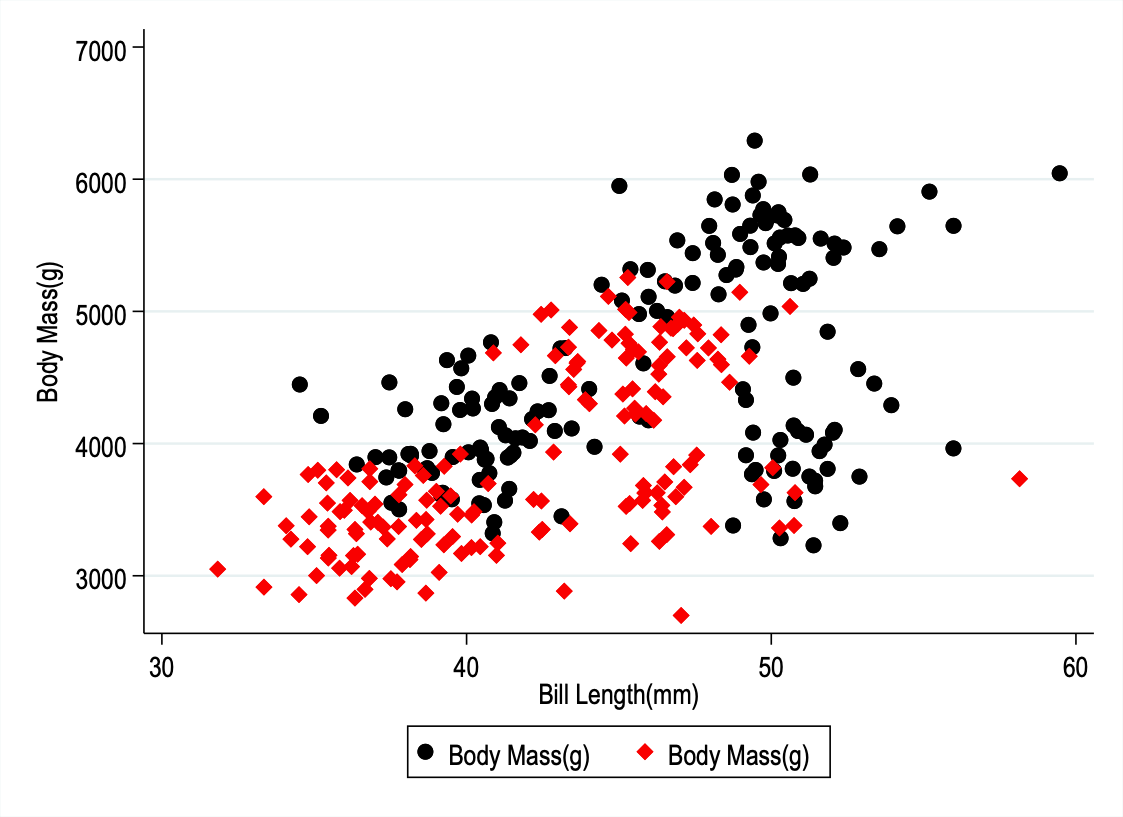
\includegraphics{penguin-sex-body_mass.png}}
  \end{center}
  \end{column}
  \hfill
  \begin{column}[T]{.5\textwidth}
  \begin{verbatim}

    tw (scatter body\_mass\_g bill\_length\_mm if sex=="male",mcolor(black) ///
    jitter(2) jitterseed(1994)) ///

    (scatter body\_mass\_g bill\_length\_mm if sex=="female", msymbol(d) mcolor(red)
    ///
    jitter(2) jitterseed(1994)), ///

    graphregion(color(white)) ///

    ylabel(,angle(360))
  \end{verbatim}
  \end{column}
  \end{columns}

\end{frame}

\begin{frame}[t]{Schemes}
  \begin{columns}
  \begin{column}[T]{.5\textwidth}
    \begin{center}
    \resizebox{0.9\linewidth}{!}{%
      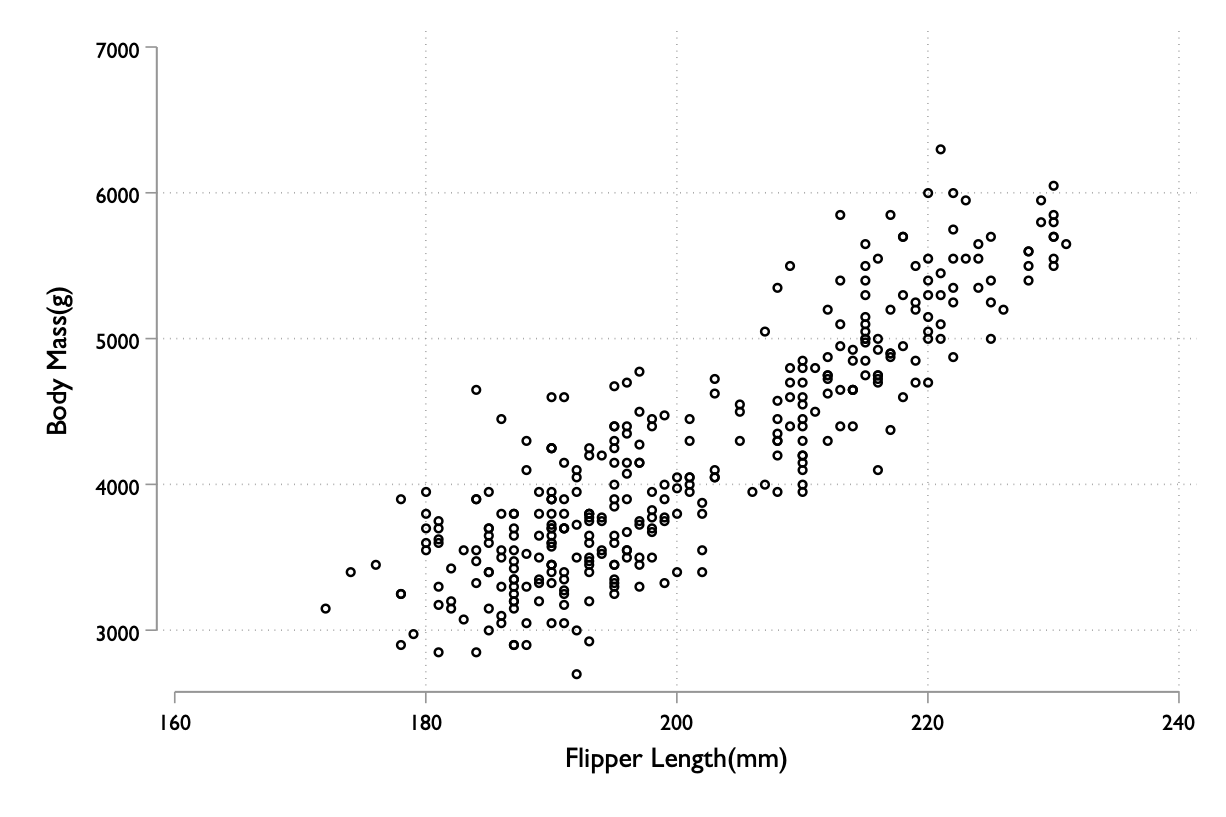
\includegraphics{theme-example.png}}
  \end{center}
  \end{column}
  \hfill
  \begin{column}[T]{.5\textwidth}
  \begin{verbatim}

tw scatter body\_mass\_g flipper\_length\_mm, mcolor(black) scheme(cleanplots)

set scheme cleanplots, perm /*sets schemes permenately */
  \end{verbatim}
  \end{column}
  \end{columns}


\end{frame}
%--- Next Frame ---%

\begin{frame}[t]{Combining Two Plots}
\begin{columns}
\begin{column}[T]{.5\textwidth}
  \begin{center}
\resizebox{0.8\linewidth}{!}{%
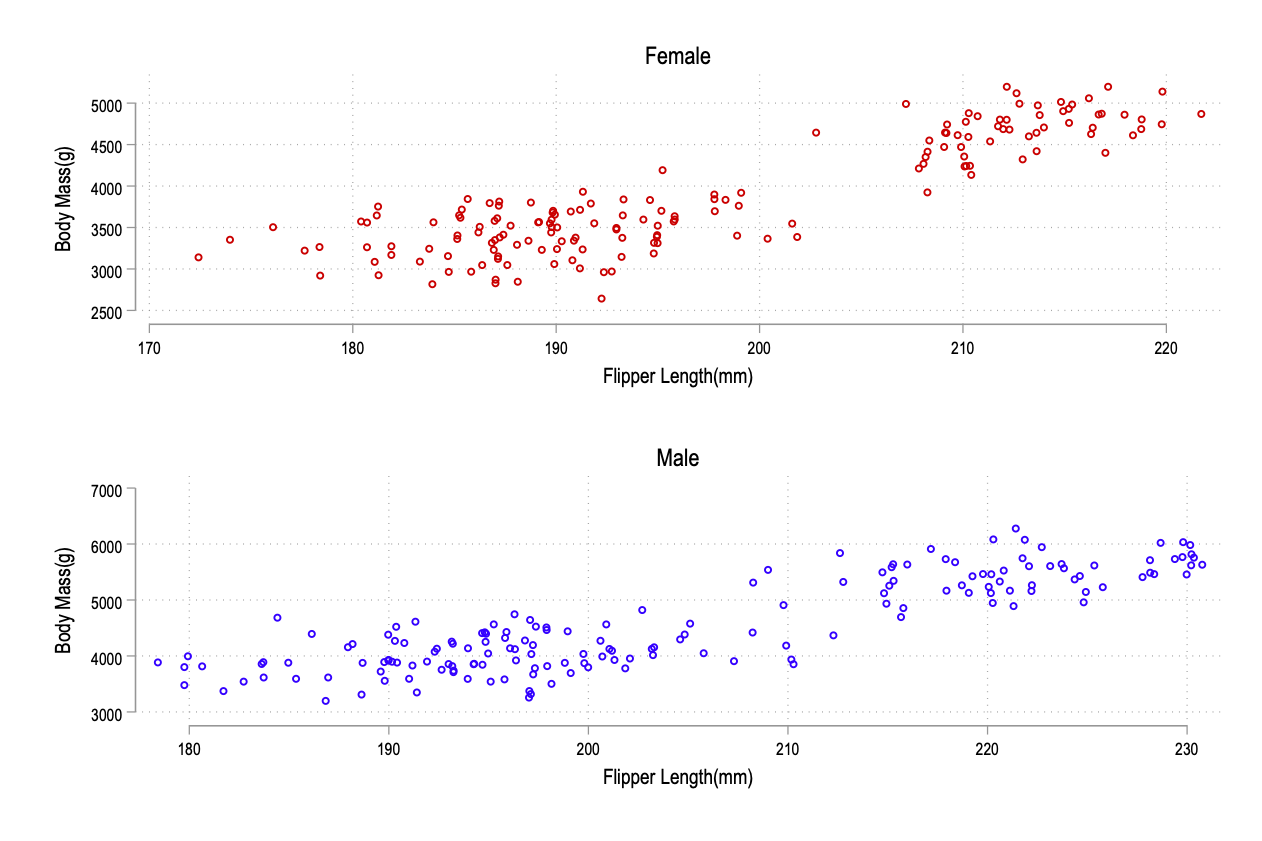
\includegraphics{combo-plot.png}
}
\end{center}
\end{column}
\hfill
\begin{column}[T]{.5\textwidth}
\begin{verbatim}

  tw scatter body\_mass\_g flipper\_length\_mm if sex == "female", jitter(2) ///
  jitterseed(1994) name(female\_scatter,replace)

  tw scatter body\_mass\_g flipper\_length\_mm if sex == "male", jitter(2) ///
  jitterseed(1994) name(male\_scatter,replace)

  gr combine female\_scatter male\_scatter, col(1)

\end{verbatim}
\end{column}
\end{columns}
\end{frame}


\begin{frame}[t]{Combining Two Different Kinds of Plots}
  \begin{itemize}
    \item We often want to convey other kinds of information
    \item You can add different kinds of plots to do this
    \item There are various ways to do this in Stata
  \end{itemize}
\end{frame}
%--- Next Frame ---%

\begin{frame}[t]{Consider This Plot}
  \begin{center}
\resizebox{.6\linewidth}{!}{%
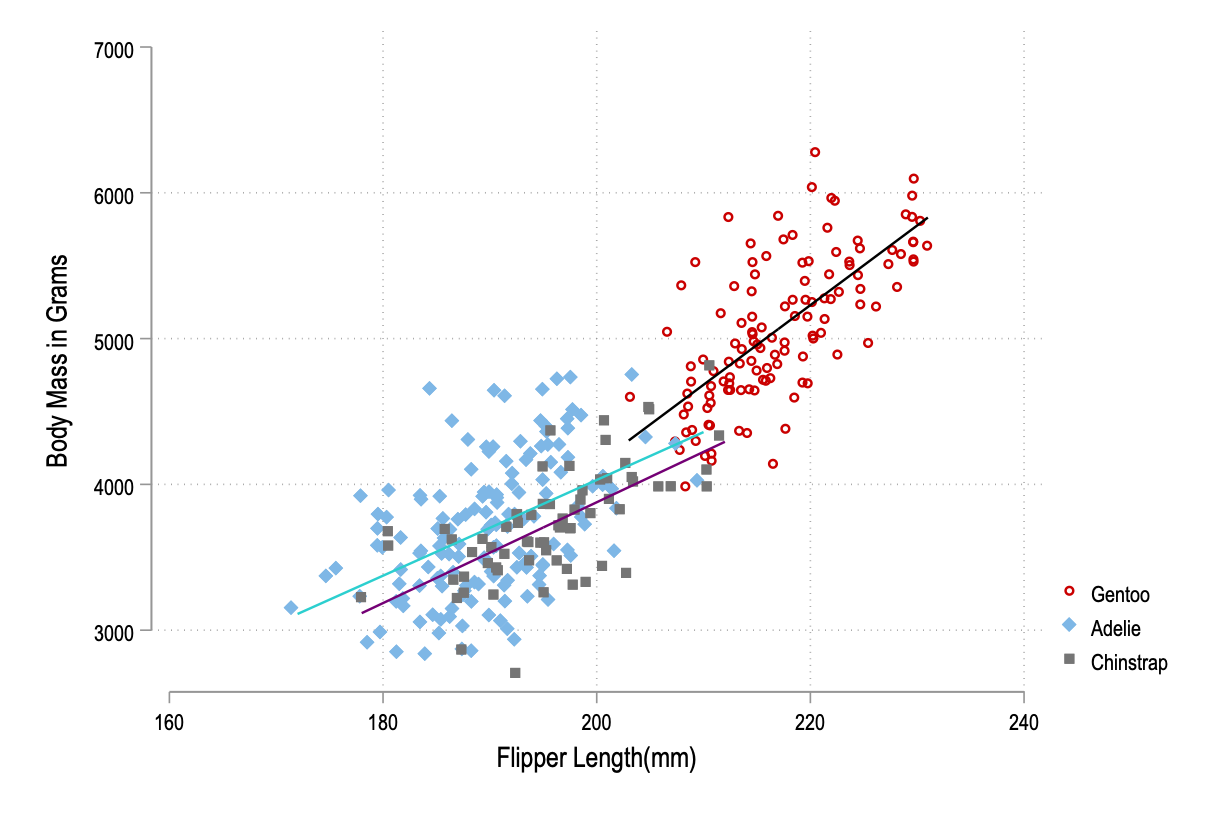
\includegraphics{multiplot-by-penguing.png}}
\end{center}
\end{frame}
%--- Next Frame ---%

\transreplace

\begin{frame}[t]{Consider This Plot}
\begin{verbatim}

  tw (scatter body\_mass\_g flipper\_length\_mm
   if species== "Gentoo", ///

   jitter(2) jitterseed(1994))  ///

  (scatter body\_mass\_g flipper\_length\_mm if species== "Adelie", ///

   jitter(2) jitterseed(1994) msymbol(d))  ///

  (scatter body\_mass\_g flipper\_length\_mm if species== "Chinstrap", ///

  jitter(2) jitterseed(1994) msymbol(s)) ///

   (lfit body\_mass\_g flipper\_length\_mm if

   species== "Gentoo") ///
   (lfit body\_mass\_g  flipper\_length\_mm if

   species== "Adelie") ///

   (lfit body\_mass\_g flipper\_length\_mm if

   species== "Chinstrap" ), ///

   legend(order(1 "Gentoo" 2 "Adelie" 3 "Chinstrap")) ///

  ytitle("Body Mass in Grams")
\end{verbatim}
\end{frame}


\end{document}
